\documentclass[PhD-Yoann-Dupont.tex]{subfiles}
\begin{document}

\begin{figure}[ht!]
\footnotesize
\begin{xml}
\xheader{xml version="1.0" encoding="UTF-8"}\\
\xmarker{master}{}{\\
  \xmarker{pipeline}{}{\\
    \xunit{segmentation}{\xfield{name}{fr}}\\
    \xunit{enrich}{\xfield{config}{pos.xml}}\\
    \xunit{label}{\xfield{model}{models/POS} \xfield{field}{POS}}\\
    \xunit{clean\_info}{\xfield{to-keep}{word,POS}}\\
    \xunit{label}{\xfield{model}{models/chunking} \xfield{field}{chunking}}\\
    \xunit{enrich}{\xfield{config}{NER.xml}}\\
    \xunit{label}{\xfield{model}{models/NER} \xfield{field}{NER}}\\
    \xunit{clean\_info}{\xfield{to-keep}{word,POS,chunking,NER}}\\
    \xunit{export}{\xfield{format}{html} \xfield{pos}{POS} \xfield{chunking}{chunking}\\
        \xfield{ner}{NER} \xfield{lang}{fr} \xfield{lang\_style}{default.css}}\\
  }\\
}
\end{xml}
\caption{une pipeline de SEM. Les pipelines permettent de définir une séquence de traitements ainsi que certaines options globales.}
\label{fig:sem-pipeline}
\end{figure}

\begin{figure}[ht!]
\footnotesize
\begin{xml}
\xheader{xml version="1.0" encoding="UTF-8"}\\
\xmarker{information}{}{\\
  \xmarker{entries}{}{\\
    \xmarker{before}{}{\\
      \xunit{entry}{\xfield{name}{word}}\\
      \xunit{entry}{\xfield{name}{POS}}\\
    }\\
    \xmarker{after}{}{\\
      \xunit{entry}{\xfield{name}{NE} \xfield{mode}{train}}\\
    }\\
  }\\
  \xmarker{features}{}{\\
    \xunit{nullary}{\xfield{name}{lower} \xfield{action}{lower} \xfield{display}{no}}\\
    \xmarker{unary}{ \xfield{name}{starts-with-upper} \xfield{action}{isUpper}}{0}\\
    \xunit{dictionary}{\xfield{name}{title} \xfield{action}{token} \xfield{path}{title.txt} \xfield{entry}{lower}}\\
    \xmarker{find}{ \xfield{name}{VerbForward} \xfield{action}{forward} \xfield{return\_entry}{word}}{\\
      \xmarker{regexp}{ \xfield{action}{check} \xfield{entry}{POS}}{\^{}V}\\
    }\\
  }\\
}
\end{xml}
\caption{exemples de fichier de génération de features de SEM, il est utilisé par le module enrich. Il permet de rajouter des descripteurs qui seront alors utilisés par les algorithmes par apprentissage automatique.}
\label{fig:sem-features}
\end{figure}


\begin{figure}[ht!]
\centering
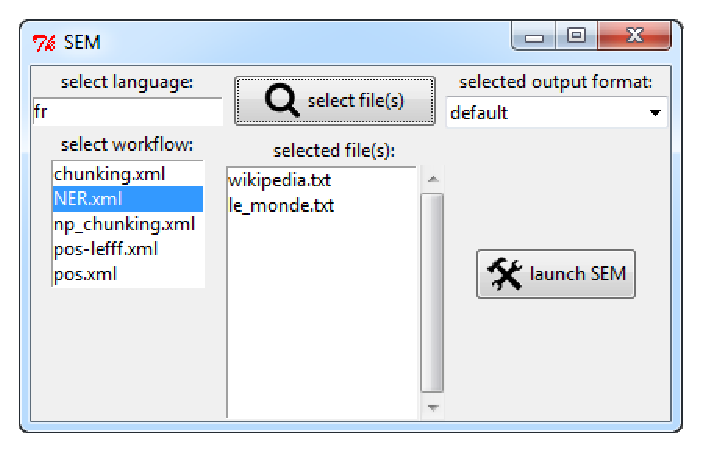
\includegraphics[scale=1.0]{images/SEM/gui}
\caption{l'interface graphique de SEM pour l'annotation.}
\label{fig:sem-GUI}
\end{figure}


\end{document}